\chapter{REQUIREMENT ANALYSIS}
\section{Hardware Requirements}
  \subsection{Raspberry Pi 4}
  The Raspberry Pi 4 is an ARM based credit card sized computer. The Raspberry Pi 4 is powered by a 64-bit quad-core ARM Cortex-A72 processor clocked at 1.5 GHZ. It has built-in wi-fi and bluetooth 5.0, making it easy to connect to the internet and other devices wirelessly.The Raspberry Pi 4 is suitable for robotics projects and Internet of Things (IoT) applications due to its GPIO pins and connectivity options. Integrating Raspberry Pi 4 in our project will leverage its processing power, and connectivity to enhance the functionality of our robotic system.
    \begin{figure}[h]
        \centering
        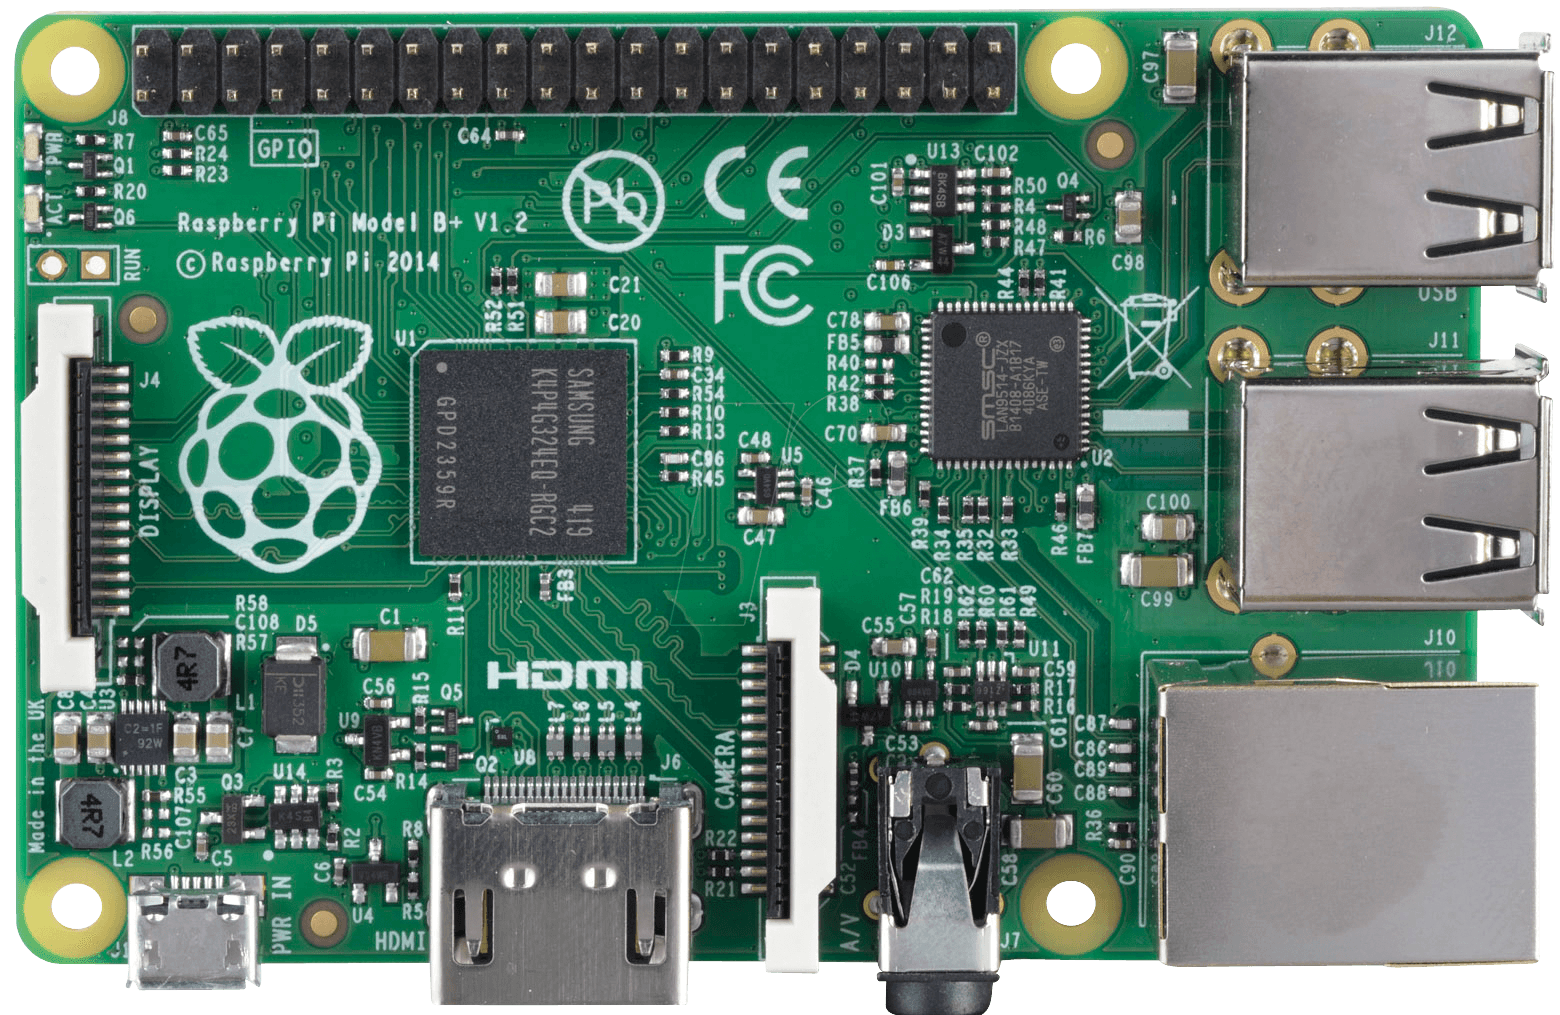
\includegraphics[width=1\linewidth]{Graphics/raspi24.png}
        \caption{Raspberry Pi 4B}
        \label{fig:enter-label}
    \end{figure}
  
  \subsection{Webcam}
  Webcam is a video camera typically connected to computer or other devices through a USB port. Webcam is used in our project to capture the robot's environment, which is essential for task like object manipulation using robotic arm. 
    \begin{figure}[h]
    \centering
    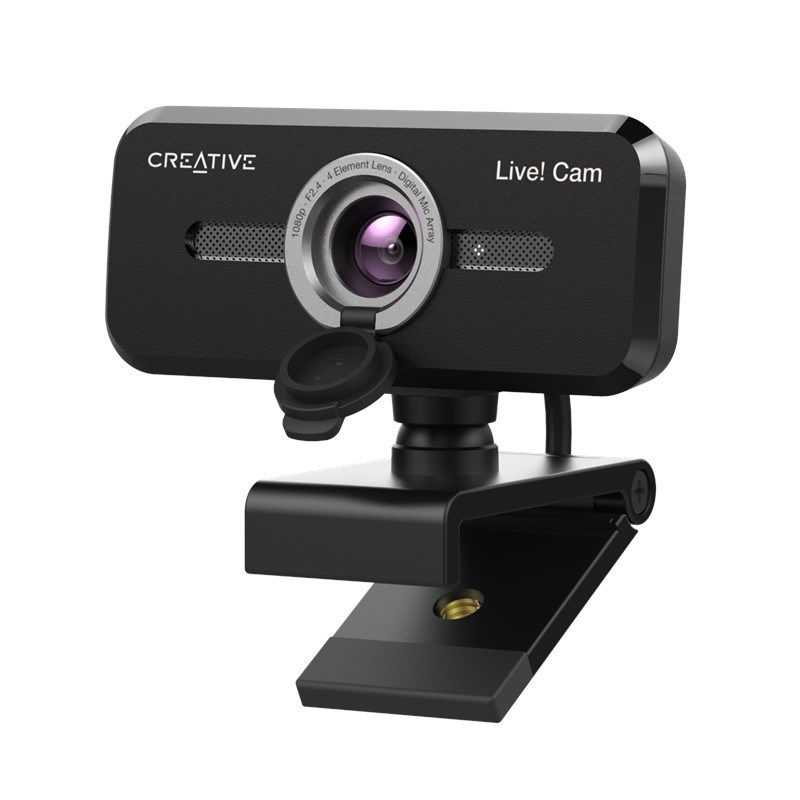
\includegraphics[width=1\linewidth]{Graphics/webcam.jpg}
    \caption{Web Cam}
    \label{fig:enter-label}
\end{figure}
  
  \subsection{MG996r Servo Motor}
  MG996r is a popular servo motor commonly used in robotics project. It is known for its high torque output, making it suitable for applications that require strong and precise movements.
  \begin{figure}[h]
    \centering
    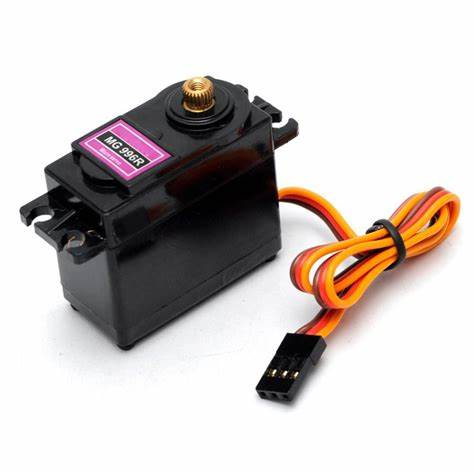
\includegraphics[width=1\linewidth]{Graphics/servoooo.jpg}
    \caption{Servo mg996R}
    \label{fig:enter-label}
\end{figure}
  \subsection{MG90s Servo Motor}
  MG90s Servo Motor is popularly known for its compact size and versatility.
  MG90s is a micro sized analog servo motor. Due to its compact size it is convenient to accommodate in small robotic projects.
  \subsection{16-Channel Servo Controller}
  A 16-channel servo controller is a device designed to control up to 16 servo motors simultaneously. Since we are using two servo motors in our project, it ensures precise control of both the servo motors.
  \subsection{Buck Converter}
  A buck converter, also known as a step-down converter, is a type of DC-DC power converter that transforms a higher voltage level into a lower one. It is able to regulate the output voltage despite the variations in the input voltage.
  \begin{figure}[h]
    \centering
    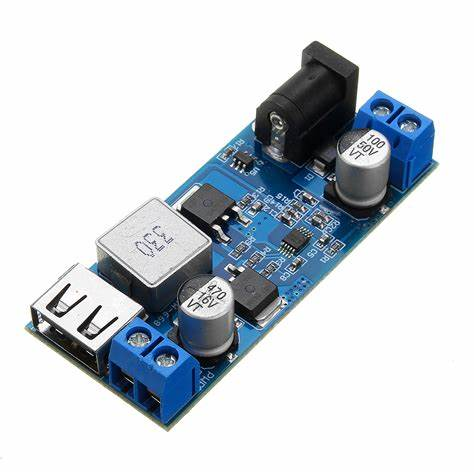
\includegraphics[width=1\linewidth]{Graphics/buckconverter.jpeg}
    \caption{Buck Converter}
    \label{fig:enter-label}
\end{figure}
\subsection{Ultrasonic Sensor}
An ultrasonic sensor works by emitting high-frequency sound waves (ultrasonic waves) and measuring the time it takes for the waves to bounce back after hitting an object. It consists of a transmitter that sends out ultrasonic pulses and a receiver that detects the echoes. By calculating the time difference between sending the signal and receiving the echo, the sensor can determine the distance to the object based on the speed of sound in the medium. Typically, ultrasonic sensors operate in the range of 20 kHz to 200 kHz, with higher frequencies providing better resolution but shorter range. They are commonly used in robotics, distance measurement, and object detection applications due to their accuracy, reliability, and non-contact nature.
\begin{figure}[h]
    \centering
    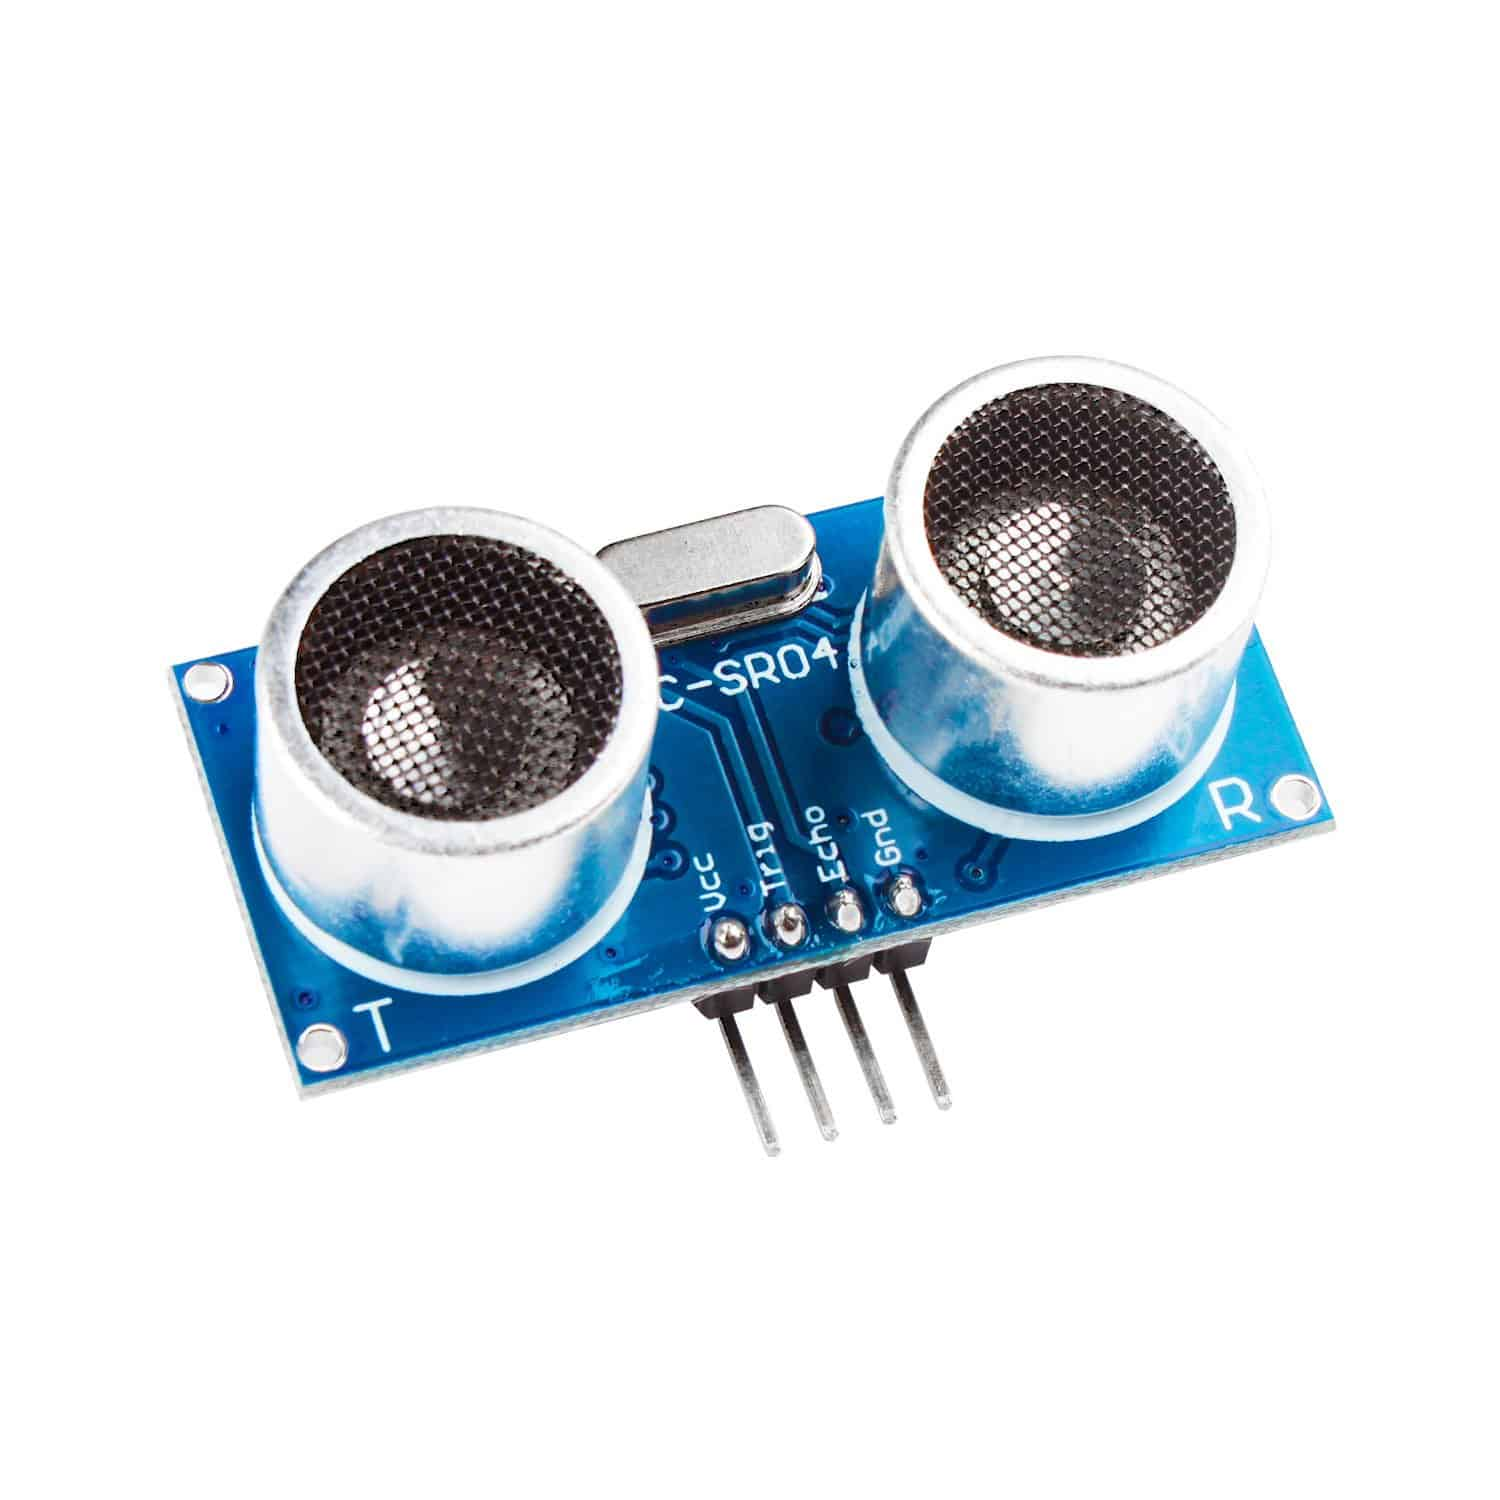
\includegraphics[width=1\linewidth]{Graphics/ultrasonicSensorImg.jpg}
    \caption{Ultrasonic Sensor}
    \label{fig:enter-label}
\end{figure}

  \section{Software Requirements}
\subsection{Python}
Python is a general-purpose language suitable for a wide range of applications, including web development, data science, artificial intelligence, automation, scientific computing, and more. Python library, SpeechRecognition was utilized to capture and interpret voice commands. Similarly, to control robotic arm and motors, to process visual data and so on Python was used in this project.
\subsection{Raspberry Pi OS(Raspbian)}
It is the official operating system designed for the Raspberry Pi single-board computers. Python is pre-installed and well-supported, making it easy for users to get started with programming on the Raspberry Pi.
\subsection{VNC Viewer}
VNC Viewer is the client application used to connect to a VNC server, enabling you to access and control the desktop of a remote system. VNC Viewer controls and access a Raspberry Pi from a desktop, laptop or mobile devices.
\subsection{VS code}
Visual Studio Code (VS Code) is a lightweight yet powerful source code editor developed by Microsoft. It offers a wide range of features tailored for software development, including syntax highlighting, code completion, debugging support, version control integration, and extensibility through a vast ecosystem of extensions. VS Code is built on the Electron framework and runs on Windows, macOS, and Linux. Its user-friendly interface, coupled with robust customization options and built-in terminal support, makes it a popular choice among developers across various programming languages and platforms. Additionally, VS Code's IntelliSense feature provides intelligent code suggestions, helping developers write code faster and with fewer errors. Overall, VS Code's versatility, performance.
